\section{Strumentazione}
	In questa esperienza si sono impiegati:
	\begin{itemize}
	\item un tetrodo a gas neon ELWE U84822330;
	\item un sistema di alimentazione e lettura di corrente ELWE;
	\item un oscilloscopio.
	\end{itemize}

Il tetrodo a gas è un tubo contenente Neon a bassa pressione in cui sono disposti 4 elettrodi che nel seguito chiameremo catodo, griglia di controllo, griglia d'anodo e collettore la cui funzione sarà  chiarita in seguito.
L'apparato fornisce la misura dei seguenti parametri:
\begin{itemize}
	\item $U_F\quad$	la d.d.p. applicata ai capi del filamento del catodo;
	\item $U_G\quad$	la d.d.p. tra catodo e griglia di controllo;
	\item $U_G\quad$	la d.d.p. tra catodo e griglia d'anodo;
	\item $U_E\quad$	la d.d.p. tra griglia d'anodo e collettore.
\end{itemize}

Si riporta in \figurename{ \ref{fig:apparato}} uno schema
	dell'apparato sperimentale impiegato.
	\begin{figure} [!h]
		\centering
		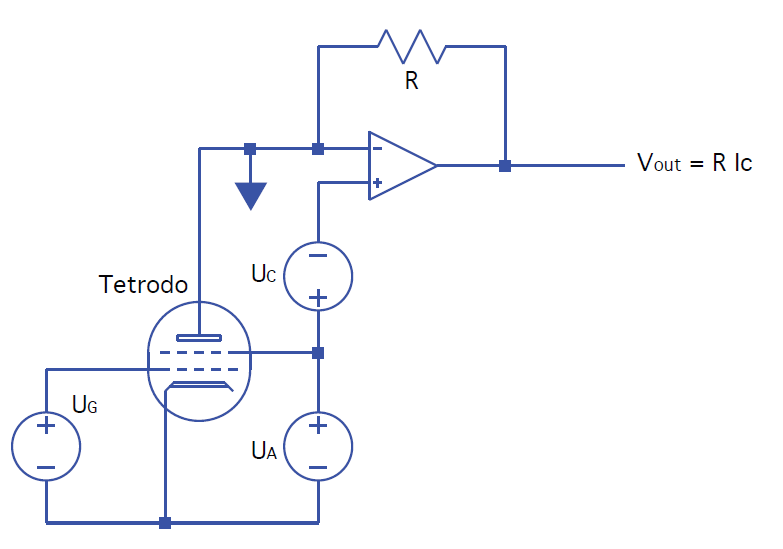
\includegraphics[width=0.5\textwidth]{apparato.png}
		\caption{Schema dell'apparato impiegato.}
		\label{fig:apparato}
	\end{figure}
